\documentclass[aps,twocolumn,showpacs,superscriptaddress]{revtex4}
%\documentclass[aps,showpacs,superscriptaddress]{revtex4}
\usepackage[pdftex]{graphicx}   % for figures
\usepackage{epstopdf}
%\usepackage{epsfig}
%draft
\usepackage{dcolumn}
\usepackage{bm}	
\usepackage{textcomp }
\usepackage{amsmath}			% Mode mathematique
\usepackage{amsfonts}			% Polices math\ufffdmatiques
\usepackage{amssymb}
\usepackage{gensymb}		% Symboles math\ufffdmatiques
\usepackage{latexsym}			% Symboles mathematiques avances
\usepackage{color}
\begin{document}

\title{Untangling resistive and collisionless electron filamentation instabilities in dense plasmas over large spatiotemporal scales}

\author{C. Ruyer}\email{charles.ruyer@cea.fr}
\affiliation{LULI - CNRS, Ecole Polytechnique, CEA : Universit\'e Paris-Saclay ; UPMC Univ Paris 06  : Sorbonne Universit\'es - F-91128 Palaiseau cedex, France}
\affiliation{SLAC National Accelerator Laboratory, Sand Hill Road, Menlo Park, California, USA}
\affiliation{CEA, DAM, DIF, F-91297 Arpajon, France}
\author{S. Bolanos }
\affiliation{LULI - CNRS, Ecole Polytechnique, CEA : Universit\'e Paris-Saclay ; UPMC Univ Paris 06  : Sorbonne Universit\'es - F-91128 Palaiseau cedex, France}
\author{B. Albertazzi}%\email{Bruno.albertazzi@polytechnique.edu}
\affiliation{LULI - CNRS, Ecole Polytechnique, CEA : Universit\'e Paris-Saclay ; UPMC Univ Paris 06  : Sorbonne Universit\'es - F-91128 Palaiseau cedex, France}
\affiliation{ INRS-EMT, Varennes, Qu\'ebec, Canada}
\author{S.N. Chen}
\affiliation{LULI - CNRS, Ecole Polytechnique, CEA : Universit\'e Paris-Saclay ; UPMC Univ Paris 06  : Sorbonne Universit\'es - F-91128 Palaiseau cedex, France}
\affiliation{Institute of Applied Physics, 46 Ulyanov Street, 603950 Nizhny Novgorod, Russia}
\author{P. Antici}
\affiliation{ INRS-EMT, Varennes, Qu\'ebec, Canada}
\author{J. B\"oker}
\affiliation{Institut f\"ur Laser-und Plasmaphysik, Heinrich-Heine-Universit\"at, D\"usseldorf, Germany}
\author{V. Dervieux}
\affiliation{LULI - CNRS, Ecole Polytechnique, CEA : Universit\'e Paris-Saclay ; UPMC Univ Paris 06  : Sorbonne Universit\'es - F-91128 Palaiseau cedex, France}
\affiliation{CEA, DAM, DIF, F-91297 Arpajon, France}
\author{ L. Lancia}
\affiliation{LULI - CNRS, Ecole Polytechnique, CEA : Universit\'e Paris-Saclay ; UPMC Univ Paris 06  : Sorbonne Universit\'es - F-91128 Palaiseau cedex, France}
\affiliation{Dept. SBAI, Universita di Roma ``La Sapienza'', Via A. Scarpa 14 00181 Rome, Italy}
\author{M. Nakatsutsumi}
\affiliation{LULI - CNRS, Ecole Polytechnique, CEA : Universit\'e Paris-Saclay ; UPMC Univ Paris 06  : Sorbonne Universit\'es - F-91128 Palaiseau cedex, France}
\author{L. Romagnani}
\affiliation{LULI - CNRS, Ecole Polytechnique, CEA : Universit\'e Paris-Saclay ; UPMC Univ Paris 06  : Sorbonne Universit\'es - F-91128 Palaiseau cedex, France}
\author{R. Shepherd}
\affiliation{LLNL, Livermore, United States}
\author{M. Swantusch}
\affiliation{Institut f\"ur Laser-und Plasmaphysik, Heinrich-Heine-Universit\"at, D\"usseldorf, Germany}
\author{M. Borghesi}
\affiliation{School Physics and Astronomy, The Queen's University, Belfast, United Kingdom}
\author{O. Willi}
\affiliation{Institut f\"ur Laser-und Plasmaphysik, Heinrich-Heine-Universit\"at, D\"usseldorf, Germany}
\author{H. P\'epin}
\affiliation{ INRS-EMT, Varennes, Qu\'ebec, Canada}
\author{M. Starodubtsev}
\affiliation{Institute of Applied Physics, 46 Ulyanov Street, 603950 Nizhny Novgorod, Russia}
\author{M. Grech}
\affiliation{LULI - CNRS, Ecole Polytechnique, CEA : Universit\'e Paris-Saclay ; UPMC Univ Paris 06  : Sorbonne Universit\'es - F-91128 Palaiseau cedex, France}
\author{C. Riconda}
\affiliation{LULI - CNRS, Ecole Polytechnique, CEA : Universit\'e Paris-Saclay ; UPMC Univ Paris 06  : Sorbonne Universit\'es - F-91128 Palaiseau cedex, France}
\author{L. Gremillet}\email{laurent.gremillet@cea.fr}
\affiliation{CEA, DAM, DIF, F-91297 Arpajon, France}
\author{J. Fuchs}\email{julien.fuchs@polytechnique.edu}
\affiliation{LULI - CNRS, Ecole Polytechnique, CEA : Universit\'e Paris-Saclay ; UPMC Univ Paris 06  : Sorbonne Universit\'es - F-91128 Palaiseau cedex, France}
\affiliation{Institute of Applied Physics, 46 Ulyanov Street, 603950 Nizhny Novgorod, Russia}

\begin{abstract}
Plasma micro-instabilities induced by high-energy particle currents play an important role in many space or laboratory plasma environments. Here, we report on measurements that reveal, over large temporal (tens of picoseconds) and spatial (hundreds of microns) scales, the growth of a multiplicity of electromagnetic filaments, following localized laser-generation of MeV electrons in a solid foil. The proton radiography data obtained in both low- and high-resistivity targets show two distinct, superimposed electromagnetic field patterns, which point to different field generation processes, namely of collisionless and resistive character. The collisionless Weibel instability is suggested, by particle-in-cell simulations, to build up in the dilute plasma expanding into the vacuum, independently of the target material, and to lead to observed azimuthally symmetric electromagnetic structures. Additionally, when the target resistivity is high enough, an additional resistive filamentation instability arises through the bulk target, resulting in observed radially elongated filaments.
\end{abstract}
\maketitle

The interaction of high-energy, charged particle flows with plasmas is a fundamental question in plasma physics and, more generally, physical kinetics. The energy and momentum transfers between the plasma species are mediated by either Coulomb collisions \cite{Shkarofsky_1966} or collective processes \cite{Belmont_2013}, depending on the density and velocity distributions of the plasma populations. Collective processes often give rise to plasma micro-instabilities, \emph{i.e.}, growing electrostatic or electromagnetic waves that develop at kinetic electron or ion scales in systems with multi-stream or anisotropic momentum distributions \cite{Davidson_1983}. 

An important class of instabilities is the Weibel-type current filamentation instability, which originates from thermal anisotropy \cite{PRL_Weibel_1959} or relative drifts between the plasma species \cite{POF_Fried_1959}. It generates small-scale electromagnetic fluctuations, which tend to deflect and thermalize the interacting particles \cite{POF_Davidson_1972, PRL_Lee_1973, APJ_Jaroschek_2004, PRL_Adam_2006}. This mechanism is drawing strong interest in high-energy astrophysics as it is suspected to underlie the creation of collisionless shocks, and their related phenomena, in weakly magnetized (electron-ion or electron-positron) plasmas \cite{RPP_Marcowith_2016}. It is also a possible mediating agent for magnetization of the intergalactic medium \cite{APJ_Schlickeiser_2003}.

Much effort is currently expended in designing experiments to investigate this instability in the laboratory, either using conventional accelerator beams \cite{PRL_Allen_2012}, or laser-generated beams \cite{PRL_Fox_2013,NP_Huntington_2015},
the latter being favored by many teams for the high-density, high-current beams that can be obtained, as well as for the variety of plasma conditions that can be simultaneously produced using auxiliary beams. 

In the case addressed here where ultraintense ($>10^{18}\,\rm W.cm^{-2}$) short ($\lesssim 1\,\rm ps$) laser pulses impinging onto overcritical targets are used to generate ultrahigh (MA) currents of energetic (MeV) electrons, the Weibel/current filamentation instability spontaneously arises from the interpenetration of these fast electrons and the background plasma. Around the laser spot, the plasma is heated to very high temperatures, and hence the instability is mainly collisionless and builds up at electron kinetic scales \cite{PRL_Adam_2006}. As of now, experimental evidence for the resulting small-scale surface magnetic fields has been obtained through high-resolution polarigrams only \cite{PNAS_Mondal_2012}. 
Fast electrons, however, can also be prone to further filamentation when propagating through the target bulk. The resistive character of the cold plasma electrons making up the fast-electron-neutralizing return current \cite{POP_Gremillet_2002} then leads to larger magnetic filaments \cite{JPP_Fiore_2010} and enhanced fast-electron scattering \cite{POP_Yang_2016}. Such resistive filamentation has been diagnosed either indirectly, from spatial modulations of the sheath-field-accelerated protons \cite{PRL_Fuchs_2003, PRL_MacLellan_2013}, or directly, from the optical emission induced by the fast electrons  \cite{PRL_Storm_2009}. Finally, the collisionless Weibel instability can also arise from fast electrons interacting with micron-scale-length plasma gradients at the target surfaces \cite{PRE_Wei_2004, PRL_Quinn_2012, PRL_Gode_2017, NJP_Scott_2017}.

\begin{figure}[tbh!]
\centerline{
\begin{tabular}{c}
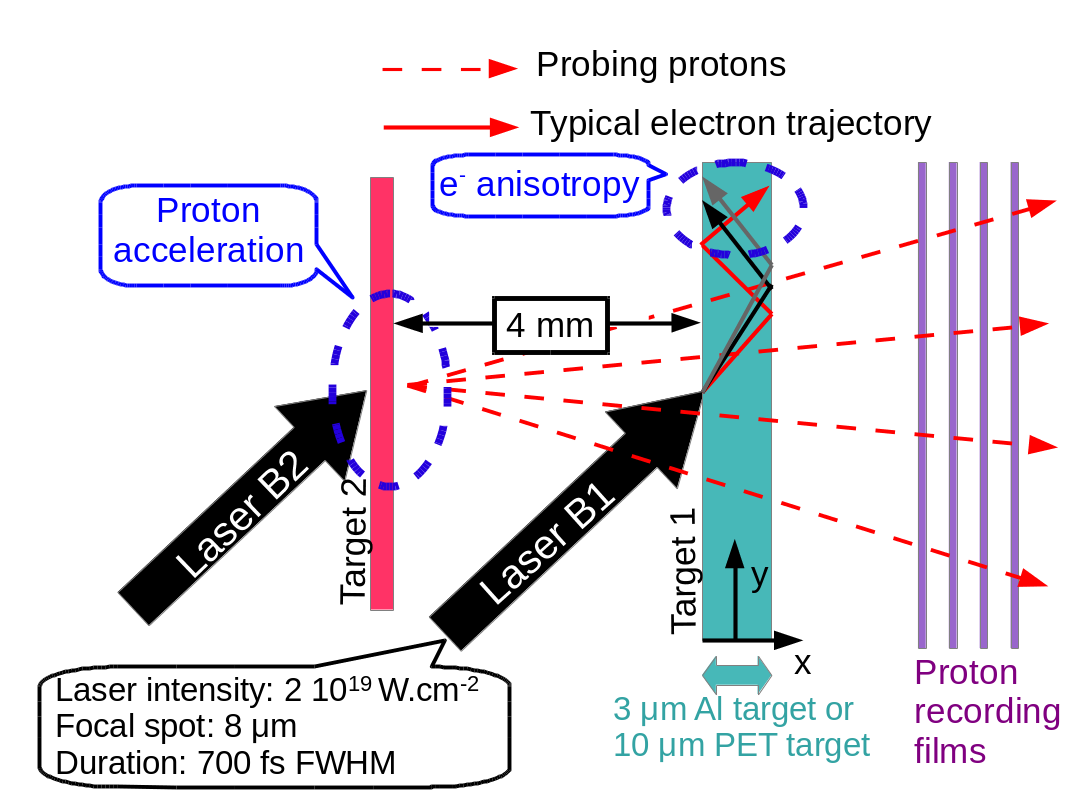
\includegraphics[scale=0.25]{sketch.png}\\
\end{tabular}}
\caption{\label{fig:xp} \textbf{Sketch of the experimental configuration and physical picture}. Target 1 is in red, target 2 in green.}
\end{figure}
The experimental and numerical data gathered so far seem to suggest that magnetic filaments only form relatively near the laser axis (over a few tens of microns), where the fast electron density, and therefore the overall plasma anisotropy, are initially at their highest. Furthermore, in contrast with simulation results \cite{POP_Heron_2015, POP_Yang_2016}, there has been as yet no observation of the simultaneous development of the collisionless and resistive variants of the instability in, respectively, the surface and inner regions of dense targets. 
Here we present measurements and simulations demonstrating: (i) filamentary magnetic-field generation by fast electrons over spatial (hundreds of microns) and temporal (tens of ps) scales much larger than previously thought possible; (ii) the simultaneous development of the collisionless and resistive types of filamentation in different areas of the target, allowing us to untangle the conditions for their occurrence.

Our measurements make use of the proton radiography technique (see Fig.~\ref{fig:xp} and Methods), by means of two high-temporal-contrast, short-pulse laser beams, B1 and B2. More details on the setup can be found in Ref.~\cite{RSI_Albertazzi_2015}.
B2 irradiates target 2 (a $3\,\rm \mu m$ thick Al or a $10\,\rm \mu m$ thick PET foil) at an angle of $31^\circ$ to the target normal, while B1 generates the probing protons from target 1. Depending on target 2's material (Al being a conductor, PET being an insulator), two types of electromagnetic field patterns are observed to arise, which kinetic simulations indicate are induced by collisionless and resistive current filamentation instabilities. These are triggered as the fast electrons, respectively, recirculate in the low-density plasma expanding into the vacuum and drift away from the laser spot into the cold, solid-density target bulk. As will be detailed in Figs.~\ref{fig:pic} and \ref{fig:kxy}, such instabilities generate electromagnetic structures consistent with the experimental observations in the Al and PET foils in terms of field strength, wavelength ($\sim 100\,\rm \mu m$), as well as spatiotemporal evolution (instability triggered a few $100\,\rm \mu m$ away from the focal spot, $\sim 4\,\rm ps$ after the main laser drive).
%
\begin{figure*}[tbh!]
\begin{tabular}{cc}
%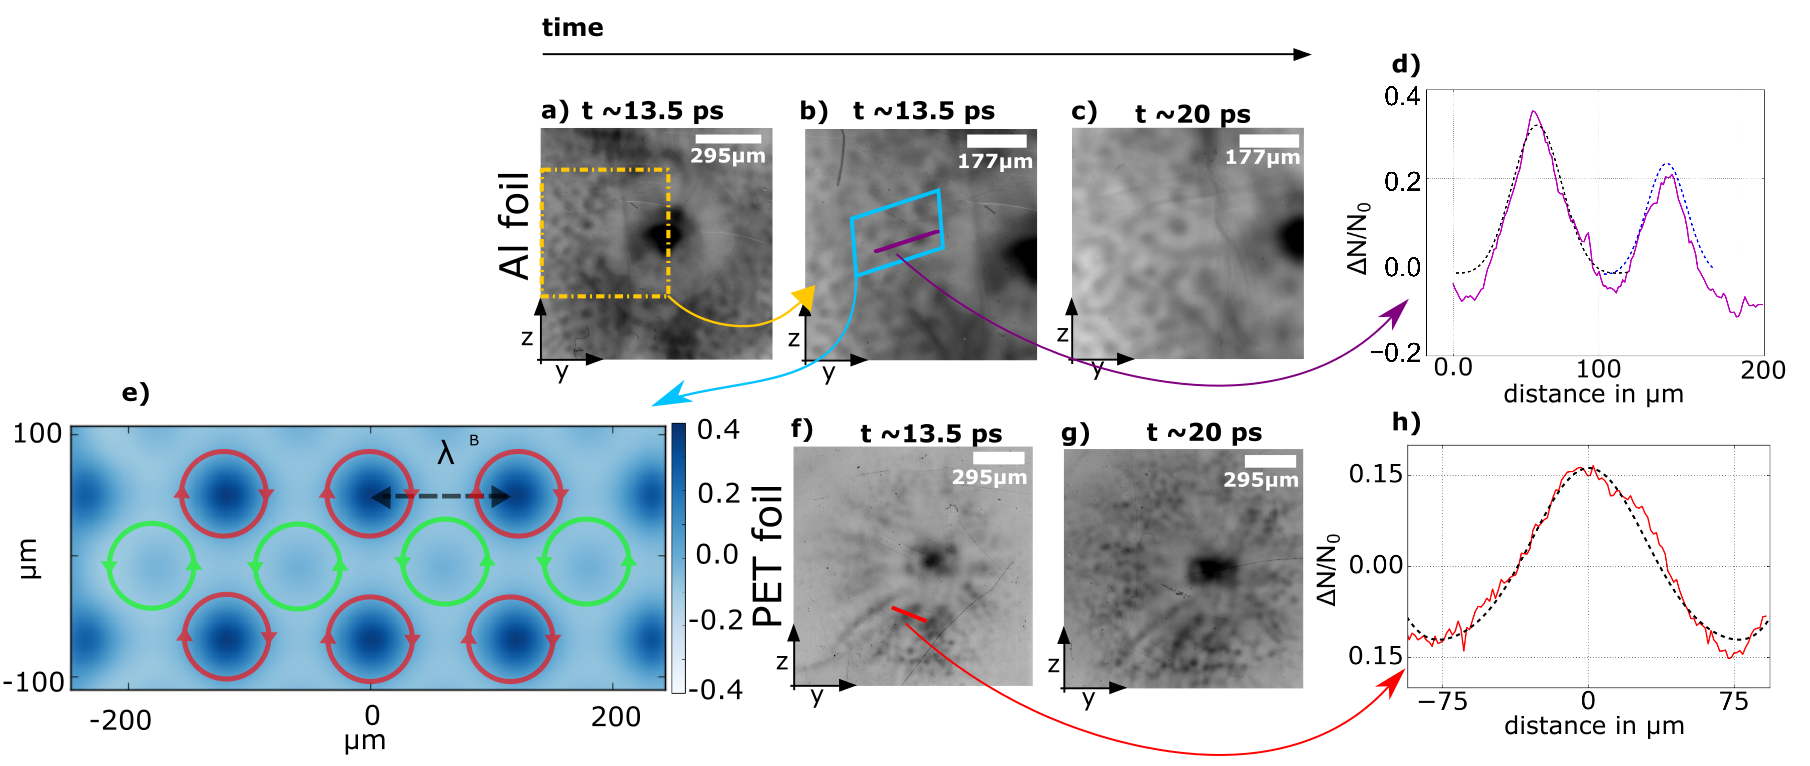
\includegraphics[scale = 0.6]{panel_v6.png}
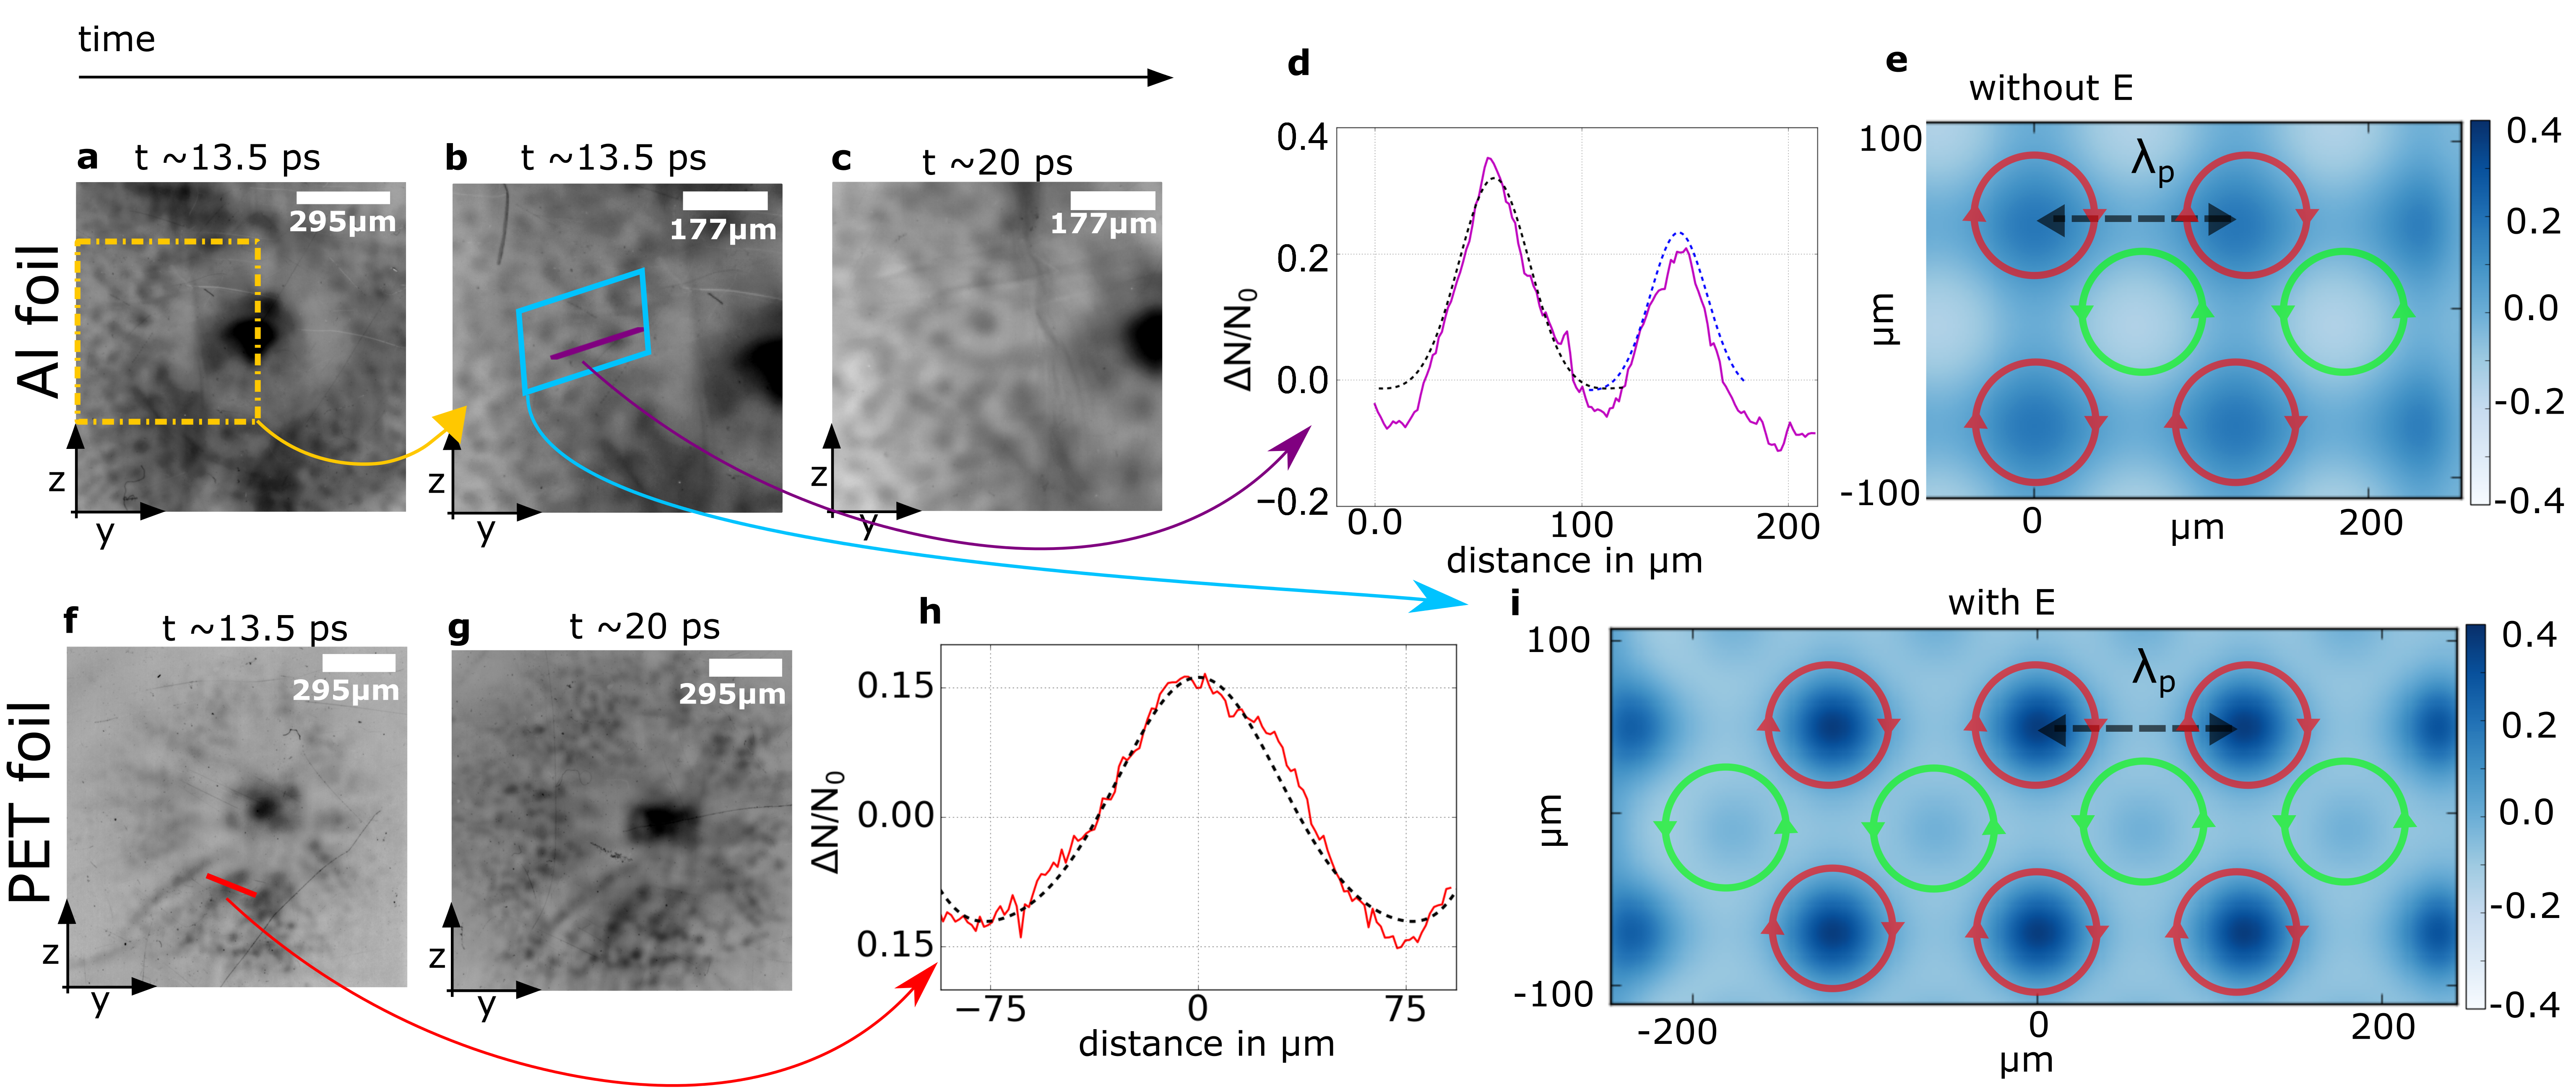
\includegraphics[scale = 0.6]{panel_v7_woE.png}
\end{tabular}
 \caption{
\textbf{Experimental proton radiographs evidencing two types of filamentation instabilities driven by hot electrons generated in solid foils, and resulting electric and magnetic field patterns, depending on the initial electrical resistivity of the target.}
\textbf{a-c}, Radiographs at various times, obtained with an Al foil as target 2. $t=0$ refers to the time at which laser B2 irradiates target 2. Darker and lighter areas correspond to increased and depleted proton dose, respectively \cite{RSI_Albertazzi_2015}. 
\textbf{b-c}, Close-ups of the off-center region delimited by the yellow dashed square in a. The small-scale modulations extending over the whole field of view are observed to develop after $\sim 1\,\rm ps$.
\textbf{d}, Proton dose profile along the purple line in b.
\textbf{e}, Schematic pattern of the magnetic (circular arrows) field lines in the zone delimited by the blue box in b, overlaid on the resulting (simulated) proton dose modulation (pseudocolor map). Red and green loops indicate magnetic field lines of opposite polarity.
\textbf{f-g}, Proton radiographs obtained with a PET foil as target 2. 
On top of a small-scale dotted pattern akin to that seen in a-c, one observes radial streaks extending from the central laser spot. 
\textbf{h}, Proton dose profile along the red line in f.
All frames, for either the Al or PET foil, corresponding to different energies of the probing protons, and hence to different times-of-flight between target 1 and target 2 (as indicated above each frame), are taken from a single shot.
\textbf{i}, Same as e but considering the additional effect of the radial electric field induced in each pinched filament (see Supplementary Information).
All spatial scales refer to the target 2 plane.}
\label{fig:radio}
\end{figure*}

On the radiographs shown in Fig.~\ref{fig:radio}, the dark and white regions result from, respectively, accumulation and depletion of the probing protons through the quasistatic fields induced around target 2. The irradiated region can be located by the large black area encircled by a white ring of $\sim 300\,\rm \mu m$ radius, delineating the large-scale $B$-field created by the Biermann battery on the surfaces of target 2 (see Ref.~\cite{RSI_Albertazzi_2015} and references therein). 
Remarkably, the radiographs also evidence a small-scale spotted pattern, developing from $\sim 400\,\rm\mu m$ to $\gtrsim 700\,\rm \mu m$ away from the focal spot, with a typical wavelength  $\lambda_p \simeq 100\,\rm \mu m$ (see lineout in Fig.~\ref{fig:radio}d).
These structures, absent without B2 irradiating target 2 (the protons then exhibit a homogeneous dose, see Fig.~2i of Ref.~\cite{RSI_Albertazzi_2015}), are observed within the first ps following the laser peak (see first frame of Fig.~2a of Ref.~\cite{RSI_Albertazzi_2015}). Moreover, they are mainly located at the bottom left-hand side of the irradiated region, \emph{i.e.}, in a domain towards which the hot electrons are expected to be preferentially flowing. Figure~\ref{fig:radio}e displays an idealized pattern of (azimuthal) magnetic and (radial) electric fields (see Methods), yielding a synthetic radiograph (pseudocolor map) qualitatively matching the experimental data. Note that the magnetic structures inferred in Ref.~\cite{PRL_Gode_2017} from modulations in the accelerated proton beam are consistent with what is observed in our radiographs, but with a much smaller wavelength and larger amplitude (due to their proximity to the laser spot).

The radiographs of the PET targets (Figs.~\ref{fig:radio}f-g) reveal a dotted pattern qualitatively similar to that seen in Al. Yet they also feature larger-scale radial dark streaks, which suggests that another mechanism for electromagnetic field generation, absent or weakly operative in Al, is here diagnosed on the line of sight of the probing protons.

\begin{figure*}[tbh!]
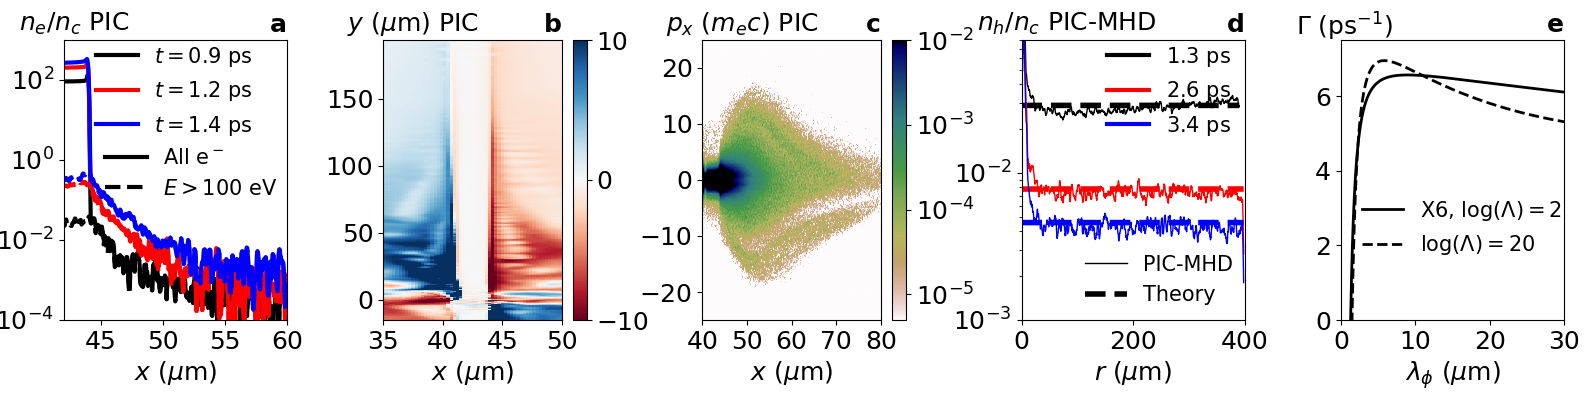
\includegraphics[scale=0.4]{Figure_3.png}
\caption{
\textbf{Numerical kinetic simulations demonstrating the occurrence of plasma conditions favorable for the growth of the collisionless and resistive current filamentation instabilities.}
\textbf{a-c}, Fully PIC 2D simulation of laser-plasma interaction in the $x-y$ plane (see Methods): 
\textbf{a}, Longitudinal lineouts at $y=117\,\rm \mu m$ of the total (solid lines) and hot ($E \ge 100\,\rm keV$, dashed lines) electron density (normalized to the critical density $n_c =1.1\times 10^{21}\,\rm cm^{-3}$) at different times, illustrating the hot-electron-driven plasma expansion along the target normal and away from the laser spot (located at $y=0$);
\textbf{b}, 2D map of the magnetostatic field $B_z$ (in $1000\,\rm T$ units, and averaged over a laser cycle)
$t =1.44\,\rm ps$ after the injection of the laser pulse on the left boundary, showing magnetic field generation in the expanding plasma as the result of the collisionless instability.
\textbf{c}, Off-axis ($y = 117\,\rm \mu m$) $x-p_x$ electron phase space at $t =1.44\,\rm ps$. Only electrons of energies $E>100\,\rm keV$ are represented.
\textbf{d}, 2D PIC-MHD simulation of hot electron transport in the $y-z$ plane (see Methods). Initial parameters are $T_{h0} = 1\,\rm MeV$, $T_{c0} = 50\,\rm eV$, $n_{h0} = 5 \times 10^{21}\,\rm cm^{-3}$, $R_0 = 32\,\rm \mu m$ and $\log \Lambda =2$. Plotted are radial lineouts of the simulated hot electron density $n_h/n_c$ (solid lines) at different times, compared with analytical estimates (dashed lines).
\textbf{e}, Theoretical growth rate $\Gamma$ (in $\rm ps^{-1}$) of the resistive current filamentation instability as a function of the poloidal wavelength $\lambda_\phi$ (see Supplementary Information). The hot electron parameters are extracted from PIC-MHD simulations run with $\log \Lambda = 2$ (solid line) and $\log \Lambda = 20$ (dashed line) at $t=0.5$ ps [$n_h \simeq 2\times 10^{19}\,\rm cm^{-3}$, $T_x \simeq 300\,\rm keV$, $T_{ec} \simeq 500\,\rm eV$, $v_r=0$,  $T_\phi = 10\,\rm keV$ (resp. $13\,\rm keV$) for $\log \Lambda =2$ (resp. 20), see Methods]. The cases of $\log \Lambda = 2$ ($\Gamma$ multiplied by 6) and $\log \Lambda = 20$ correspond to conducting and insulating targets, respectively.}
\label{fig:pic} 
\end{figure*}

We will now show that the recirculation of the hot electrons across the dilute plasma expanding from the target surface triggers collisionless current filamentation, thus giving rise to electromagnetic structures such as those sketched in Fig.~\ref{fig:radio}e. In order to investigate the large-scale hot electron dynamics in a self-consistent way, we have performed a 2D particle-in-cell (PIC) simulation using the code \textsc{calder} \cite{NF_Lefebvre_2003}. This simulation describes the laser-plasma interaction (and related collisional and ionization processes) in the $x-y$ plane shown in Fig.~\ref{fig:xp}, with half-reduced Al density to alleviate the computational effort (see Methods).
We see in Fig.~\ref{fig:pic}a that, already after $1.44\,\rm ps$ of laser plasma interaction, the rear target surface has expanded a distance $>10\,\rm \mu m$, and that magnetic modulations have developed in the expanding plasmas from the two target sides (see Figs.~\ref{fig:pic}b, S1 and  Figs.~S7a,b in the Supplementary Information). At the target backside ($x>44\,\rm \mu m$), they extend up to $y \lesssim 150\,\rm \mu m$ from the laser spot, with a typical wavelength $\lambda_p \sim 6\,\rm \mu m$.

\textcolor{blue}{The $x-p_x$ electron phase space extracted along $y = 117\,\rm \mu m$ shown in Fig.~\ref{fig:pic}c reveals the overlap of the expanding hot electrons  with a counterstreaming population. A momentum-flux anisotropy is also evidenced in Fig.~S1f, of the order of $1$, suggesting that the expanding region is unstable to Weibel-type instabilities \cite{POP_Ren_2006, PRL_Gode_2017}. Growth rate and wavelength estimates may be obtained resolving the dispersion relation  for an \emph{ad-hoc} two-temperature relativistic distribution function (see Supplementary Information, Sec. II) which parameters may be fitted on our fully PIC simulation results.
The approximate magnetic-field wavelength and strength (see Supplemental information Sec. V.A) are related to the hot electron plasma frequency, $\omega_{ph}=\sqrt{n_h e^2/m_e \epsilon_0}$, through 
\begin{align}
  \lambda_p &\simeq \alpha_\lambda 2\pi c/\omega_{ph} \label{eq:lp}  \,,\\
  B_p &\simeq \alpha_\Gamma^2\alpha_\lambda m_e \omega_{ph}c/ ev_h \label{eq:bp} \,, 
\end{align}}
where $c$, $\epsilon_0$, $n_h$, $m_e$ and $e$ are the speed of light in vacuum, the vacuum permittivity, the hot electron density, the electron mass and  charge, respectively. \textcolor{blue}{Moreover, $\alpha_\lambda $ and $\alpha_\Gamma $ are proportionality factors mainly depending on the anisotropy and the energy of the  electron distribution  which  in our case reads $\alpha_\lambda\sim 2 $ and $\alpha_\Gamma\sim 0.1 $ (see Supplementary Information).
Additionally, a radial electric field (see Fig. S1c) $E_p \simeq - \nabla B_p^2/(2 \mu_0e n_h)$ arises from charge separation between the magnetically pinched electrons and the ions in the vicinity of the filament \cite{POP_Dieckmann_2009, POP_Bret_Gremillet_2010}. 
Using Eqs.~\eqref{eq:lp} and \eqref{eq:bp}, its typical strength is 
\begin{align} 
  E_p \simeq \alpha_\Gamma^4  \alpha_\lambda^2 m_ec^3\omega_{ph}/2ev_h^2 \label{eq:ep} \, .
\end{align}}
While the magnetic field around a filament may be focusing or defocusing (regarding the probing protons) according to the filament's current sign, the accompanying electric field is always focusing. The net effect on the proton deflection is found to depend on the modulation wavelength $\lambda_p$ (see Supplementary Information, Sec. V.B).

In order to demonstrate that the instability seen to grow in the simulated expanding plasma (Fig.~\ref{fig:pic}b) accounts for the dotted pattern evidenced by the radiographs (Fig.~\ref{fig:radio}), we have to disentangle the impact of the reduced geometry of our simulation on the hot-electron dynamics. Indeed, unlike in Refs.~\cite{PRL_Gode_2017, NJP_Scott_2017}, field modulations here build up at least a picosecond after the laser irradiation, and hundreds of microns away from the focal spot, where multidimensional electron dilution effects should arise. Obviously, such effects are improperly treated in our fully PIC 2D simulation, which resolves only the $x-y$ plane. Yet they can be evaluated by estimating the temporal evolution of the hot-electron density, $n_h$, in a general system of spatial dimension $D+\delta$, where $D$ and $\delta$ denote the number of dimensions in the target plane and normally to it, respectively. Assuming a homogeneous distribution over the hot-electron light cone, and taking into account both the transverse thermal spread of the hot electrons and the longitudinal plasma expansion, one obtains $n_h(t) \simeq n_{h0}/(1+ v_h t /R_{h0})^D/(1+c_{sh} t/L)^\delta$ with $L$, $c_{sh}$, $n_{h0}$ and $R_{h0}$ being the target thickness, sound speed and initial hot-electron density and  deposition radius (see Supplementary Information).
\textcolor{red}{Que vaut $v_h$ ? En pratique, il devrait plut\^ot s'agir de $\langle v_\perp \rangle \simeq c\sin \theta \simeq c/3-c/2$, non ?}
\textcolor{blue}{From the simulation we estimate $R_{h0} \simeq 32\,\rm \mu m$ at the time of the maximum hot-electron density $n_{h0} \simeq 5\times 10^{21}\,\rm cm^{-3}$. The above formula with $D=\delta=1$ gives an average density $n_h \simeq 8 \times 10^{19}\,\rm cm^{-3}$ at $t = 1.44\,\rm ps$ \textcolor{red}{(quelle origine des temps ?)}, consistent with Fig.~\ref{fig:pic}a. Further, Eqs.~\eqref{eq:lp}-\eqref{eq:ep} predict $\lambda_p \simeq 4 \,\rm \mu m$, $B_p \simeq 510\,\rm T$ and $E_p \simeq 2.4\times10^{10}\,\rm Vm^{-1}$, close to the simulation results (see Fig.~\ref{fig:pic}b and S7a). In the experiment ($D=2$, $\delta=1$), at the time of the first observation ($t=4\,\rm ps$),
\textcolor{red}{(on voit d\'ej\`a des choses \`a $t=1\,\rm ps$)} we obtain
$\lambda_p \simeq 58 \,\rm \mu m$ \textcolor{red}{(\`a corriger)}, consistent with the structures observed in Figs.~\ref{fig:radio}a-c, and $B_p\simeq 24\,\rm T$ \textcolor{red}{(\`a corriger ?)}, also comparable with the experimentally inferred value of $\sim 10\,\rm T$ (see Methods). One also expects an electric field strength $E_p \simeq 1.5\times 10^9\,\rm V m^{-1}$, high enough to affect the radiographs (see Fig.~\ref{fig:radio}i) by increasing (resp. fading) the contrast of the focusing (resp. defocusing) magnetic loops (see Supplementary Information). Finally, at late times, hot electron recirculation and target expansion should occur on both sides of the target, possibly leading to two independent electromagnetic patterns superimposed, by the probing protons, on the detector.}

%This estimate remains valid far from the irradiated region after the laser has deposited its energy
Moreover, we have carried out a series of 2D PIC-MHD simulations resolving, in the $y-z$ plane, the hot-electron lateral transport through the collisional solid-density Al target. In these simulations, the laser-plasma interaction and longitudinal plasma expansion are not described, while the response of the thermal bulk electrons is modeled in the resistive MHD limit, which allows the hot electrons to be followed over larger spatiotemporal scales than in the fully PIC simulation (see Methods). The hot electrons are initialized as an isotropic Maxwellian population of temperature $T_{h0}=1\,\rm MeV$ and density $n_{h0}=5\times10^{21}\,\rm cm^{-3}$, contained in a circular region of radius $R_{h0}=32\,\rm \mu m$. The initial Al plasma temperature is of $50\,\rm eV$, corresponding to a $5+$ ionization degree. Such input parameters are based on the fully PIC simulation data (see Supplementary Information). The resulting hot-electron density profiles, plotted at various times in Figs.~\ref{fig:pic}d and S7a,b, support the above estimate for $n_h(t)$ (taking $D=2$ and $\delta=0$).

\begin{figure*}
\centerline{
\begin{tabular}{ccc}
\textbf{a} PIC-MHD magnetic field  &  \textbf{b} Synthetic radiograph without expanded plasma  &  \textbf{c} Synthetic radiograph  \\
&  &   with expanded plasma \\
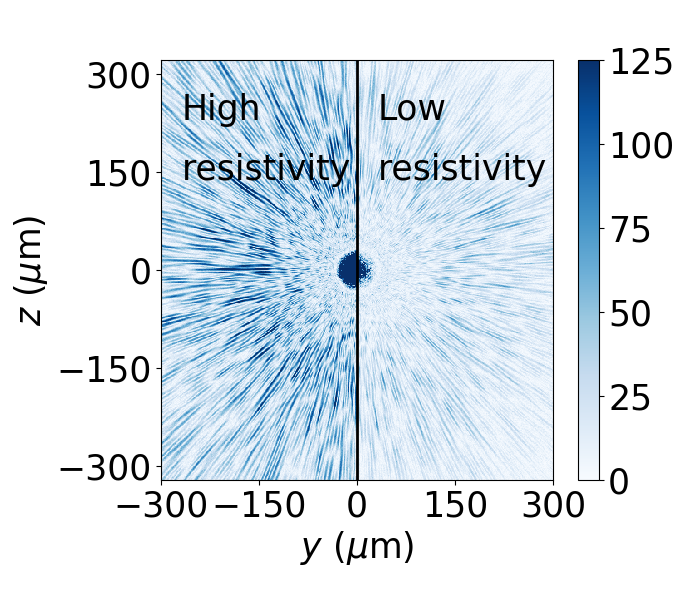
\includegraphics[scale=0.33]{B_Te0_05_ne300_nh5_Th1MeV_t10500_complog.png} &
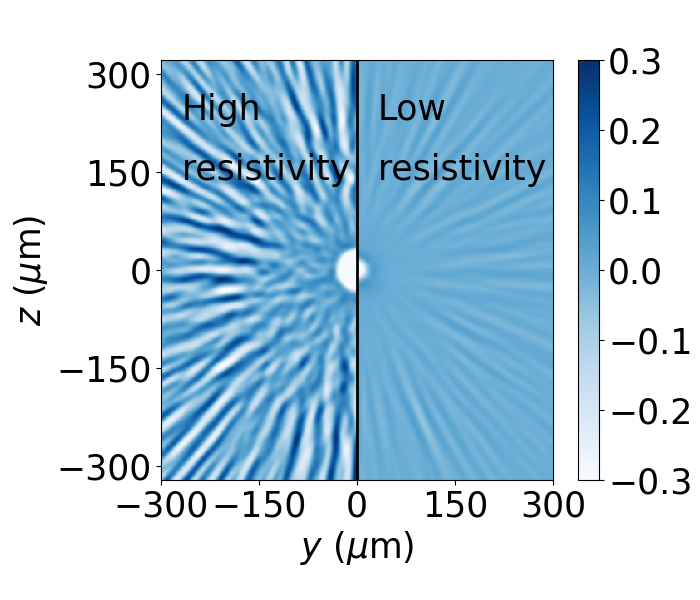
\includegraphics[width=0.33\textwidth]{DN_Te0_05_ne300_nh5_Th1MeV_t10500_complog_300mum.png} &
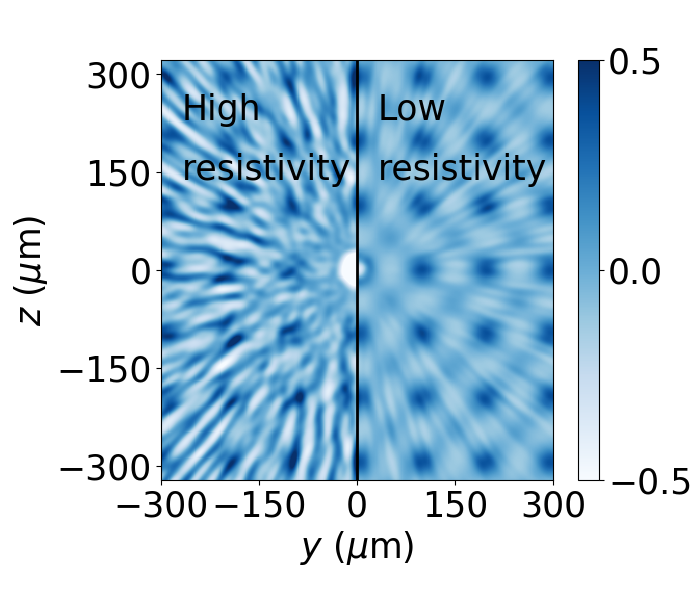
\includegraphics[width=0.33\textwidth]{DN3D_complog_R20_a60_l140.png}
\end{tabular}}
\caption{
\label{fig:kxy}
\textbf{2D PIC-MHD simulations evaluating the resistive filamentation growth in the solid foil plane for various initial electrical resistivities.}
\textbf{a}, Magnitude of $B_\perp=(B_x^2+B_y^2)^{1/2}$ (in Teslas) at time $t=3.28$ ps for $\log \Lambda=20$ (\emph{i.e.} modeling an insulator, $y<0$) and $\log\Lambda=2$ (\emph{i.e.}, modeling a conductor, $y>0$).
\textbf{b}, Synthetic radiographs from $8$ MeV probing protons in a 
$3\, \mu$ m thick target with B-fields given by a, see Methods.
\textcolor{red}{
\textbf{c}, Synthetic radiographs with superimposed filaments extending in the $z$ direction over $L_p = 48\,\mu$m, see Methods.} 
The magnetic field profile used for the reconstruction is poloidal around each filament center following Fig.~\ref{fig:radio}e with $\lambda_p = 120\, \mu$m, and with a radial profile given by Eq.~\eqref{eq:bloop} with $B_0=10$ T and $a = 60\, \mu$m. Two electromagnetic distributions have been placed on the expanding front and rear sides of the $3\,\mu$m thick target.
}
\end{figure*}

The PIC-MHD simulations capture the lateral spreading dynamics of the hot electrons, and hence the resistive filamentation instability that can affect it. As the electrons move radially away from their generation region, their momentum distribution becomes ``cold'' in the poloidal ($\theta$) direction, while it stays ``hot'' along the other ($r,x$) directions (see Fig.~S6 in Supplementary Information Sec. IV). A large hot electron pressure anisotropy is therefore driven in $\sim 0.5\,\rm ps$, although its final level may be overestimated due to neglect of the longitudinal target expansion and of the associated electron-to-ion momentum-transfer (occurring after $\sim L/2c_{sh} \sim 0.5\,\rm ps$ \cite{PRE_Mora_2005}). Therefore, in the case of the conducting Al target (characterized by a Coulomb logarithm $\log \Lambda = 2$ \cite{POF_Lee_1984}), a non-propagating magnetic modulation builds up after a few $100\,\rm fs$ (see \mbox{Fig.~\ref{fig:kxy}a, right}), reaching a field strength $\langle B_\phi^2\rangle^{1/2}\simeq 34\,\rm T$ (averaged over the region $100 \ge r \ge 200\,\mu \rm m$) with a typical wavelength $\lambda_\varphi \simeq 5-10\,\rm \mu m$  in the poloidal direction. Those results are consistent with the linear dispersion relation of the resistive filamentation instability, evaluated using parameters extracted from the PIC-MHD simulation at $t=0.5\,\rm ps$, and which predicts a fastest-growing wavelength $\lambda_\phi \simeq 5\,\mu \rm m$ (Fig.~\ref{fig:pic}e, see Supplemental Information Sec. III). The instability growth time, $\Gamma_\phi^{-1}\simeq 160\,\rm fs$ also agrees with the experimental time of appearance of the proton dose modulations ($0-1\,\rm ps$ after laser irradiation).

We will now evaluate the influence of the target electrical resistivity on the observed radial structures. The hot-electron dynamics into the insulating PET target is expected to differ from that in the conducting Al target due to higher electrical resistivity at low temperatures \cite{PRL_Fuchs_2003,PRL_McKenna_2011}. Since our PIC-MHD framework ceases to be predictive outside the Spitzer collisional regime ($T\lesssim 50\,\rm eV$), we will restrict ourselves to a qualitative comparison by running the same simulation than in Al but with an artificially enhanced resistivity, \emph{i.e.}, using a Coulomb logarithm $\log \Lambda = 20$ instead of $\log \Lambda = 2$, so as to to mimic the response of the PET target. Comparing the magnetic field maps displayed in the left and right sides of Fig.~\ref{fig:kxy}a, one can see that about twice stronger field modulations ($\langle B_\phi^2 \rangle^{1/2} \simeq 70\,\rm T$ vs. $35\,\rm T$) build up at $\log \Lambda = 20$, while keeping approximately the same wavelength. This behavior is consistent with the theoretical dispersion relation of the resistive filamentation. Using the simulation data in the region $50 \le r \le 100\,\rm \mu m$ (see Figs. S6a-f), the maximum growth rate (dashed line in Fig.~\ref{fig:pic}e) is predicted to be $\sim 6$ times larger at $\log \Lambda = 20$ than at $\log \Lambda = 2$, with about the same wavelength.

After saturation of the instability, the hot electrons' contribution to the self-induced magnetic structures progressively weaken due to dilution, so that they end up being sustained by the bulk thermal electrons only, and thus being subject to magnetic diffusion over a timescale $\sim \mu_0 \sigma \lambda_\phi^2 \gtrsim 30\,\rm ps$ at temperatures $\gtrsim 50\,\rm eV$. Hence, we do not expect significant evolution of the fields inside the target over a few $10\,\rm ps$ following the final simulation time ($3.28\,\rm ps$).

Figures~\ref{fig:kxy}b,c display synthetic radiographs obtained from proton ray-tracing calculations through the field distributions extracted from the above simulations (see Methods). In Fig.~\ref{fig:kxy}b only the PIC-MHD fields are taken in account (for both $\log \Lambda =2$ and $\log \Lambda = 20$), while Fig.~\ref{fig:kxy}c further considers the effect of the electric and magnetic fluctuations that arise in the expanding plasma (as predicted by the fully PIC simulation). In all cases, scattering of the probing protons off the target ions is also described (see Methods and Supplementary Information Sec. V), and is responsible for the smoothed rendering of Fig.~\ref{fig:kxy}b compared to Fig.~\ref{fig:kxy}a. In the low-resistivity (Al) target,  Figs.~\ref{fig:kxy}b,c show that the dotted field pattern generated in the expanding plasma mainly accounts for the observed proton modulations. In the high-resistivity (PET) target, by contrast, the field patterns generated both in the expanding plasma and in the bulk target are found to contribute to the radiographs. The fact that
the experimental radiographs in PET (Figs.~\ref{fig:radio}f,g) exhibit about twice fewer radial structures than the synthetic radiograph (Fig.~\ref{fig:kxy}b) can be ascribed to the crude modeling of the electrical resistivity of the target and to uncertainties in the initial hot electron parameters.

To conclude, we have shown, through proton radiography, that the energetic electrons generated by an intense short-pulse laser can induce quasistatic electromagnetic fluctuations at surprisingly large distances (a few hundreds of $\rm \mu m$) from the laser spot. Based on kinetic simulations and analytical estimates, our analysis reveals that two instability-based mechanisms for field generation can operate simultaneously, namely collisionless current filamentation in the expanding plasmas formed at the target surfaces, and resistive current filamentation in the bulk target. The former is found to prevail in conducting Al targets, while both yield comparable field strengths in high-resistivity PET targets. A full quantitative understanding of our experimental observations would require describing the multidimensional hot-electron kinetics in dense plasmas over tens of ps and hundreds of $\rm \mu m$ spatiotemporal scales. Not only out of reach of state-of-the-art kinetic simulation codes, this challenging problem would also involve progress in the theoretical modeling of the coupled-to-weakly-coupled plasma transition during laser irradiation.

\section*{Methods}
\subsection*{Experiments}
The experiment 
was performed at the Jupiter Laser Facility's \textsc{titan} laser at the Lawrence Livermore National Laboratory \cite{RSI_Albertazzi_2015}. Each laser beam B1 and B2 had an energy of $55\,\rm J$ ($\pm 10\%$), a pulse duration of $\sim 700\,\rm fs$ FWHM, and was focused with a $f/3$ parabola at $31^\circ$ incidence angle, resulting in an on-target intensity of $\sim 2\times 10^{19}$ W.cm$^{-2}$. The normalized laser field strength is $A_0 = eE/m_ec\omega_0 \simeq 4$, where $\omega_0$ is the laser frequency. Before focusing, B2 was reflected off a plasma mirror, with $70\,\%$ efficiency, in order to improve its temporal contrast \cite{PRE_Doumy_2004}. A high temporal contrast ensures steep density gradients at the target surface, which is critical for the formation and observation of the far-distant magnetic loop structures revealed here (\emph{e.g.}, compare with the results of Ref.~\cite{PRL_Sarri_2012} where no similar structures are observed, likely due to the generation of a large preplasma by the laser prepulse). Under our high-temporal-contrast and oblique-incidence conditions, hot electron generation is expected to be dominated by the so-called ``vacuum heating'' mechanism \cite{PRE_May_2011}. After $700$ fs, when the laser-intensity drops, a significant fraction ($\sim 50\,\%$ \cite{PRL_Ping_2008}) of the $\sim 55\,\rm J$ laser energy has been converted into a total number of $\sim 10^{14}$ hot electrons.

The probing protons, generated through target normal sheath acceleration \cite{PRL_Fuchs_2003} by focusing B1 onto a $50\,\rm \mu m$-thick Au foil, had a useful energy range of $4.5\,\rm MeV$ to $9.5\,\rm MeV$. They probed the $B$-fields developing in target 2 in a ``face-on'' configuration \cite{RSI_Albertazzi_2015}, suited to measuring toroidal magnetic loops having their axis along the target normal, while minimizing the influence of the $E$-fields that develop along the target normal. As shown in Fig.~\ref{fig:xp}, the probing protons, after propagation through target 2, were collected by a stack of radiochromic films in which they were stopped in distinct layers according to their incident energy. Time-of-flight differences between protons of various energies from their source up to target 2 allowed us to probe the central, large-scale, as well as the radially distant, smaller-scale, electromagnetic fields at successive times ($t=0$ corresponds to the time at which B2 strikes target 2). Target 2 was either a $3\,\rm \mu m$-thick Aluminium (Al) foil or a $10\,\rm \mu m$-thick Polyethylene terephthalate [PET, an insulator polymer with composition $(\mathrm{C}_{10}\mathrm{H}_8\mathrm{O}_4)_n$].
 
\subsection*{2D fully PIC simulation}

A large-scale PIC simulation (2D in space, 3D in momentum) of the irradiation of the Al foil by the laser beam B2 has been performed using the PIC code \textsc{calder}. The laser beam has a Gaussian temporal profile of $690$ fs FWHM, a Gaussian spatial profile of $8\, \mu$m FWHM and a $30^\circ$ incidence angle. Its maximum intensity is of $3.5 \times 10^{19}$ W.cm$^{-2}$, reached at $t=1.3$ ps at the left-hand side of the domain. The target is composed of three layers: H$^+$ ($0.7\,\mu$m), Al$^{3+}$ ($3.7\,\mu$m) and neutral hydrogen ($6$ nm). Its density profile consists of a $3\, \mu$m long plateau preceded by a $1.4\,\mu$m-long preplasma made of H$^+$ and Al$^{3+}$ ions. The maximum ion target density is taken to be half the solid density ($n_\mathrm{Al}=n_\mathrm{H}=90 n_c$) so as to reduce the computational load. All species are initialized with a temperature of $10$ eV.

The numerical box has dimensions $L_x \times L_y = 48 \times 278\,\rm \mu m^2$ with a spatial discretization $\Delta x = \Delta y = 5.6\,\rm nm$ and a time step $\Delta t = 1.48\times 10^{-2}\,\rm fs$. An alternating-order interpolation scheme \cite{CPC_Sokolov_2013} is employed with a 4th-order weight factor. Each cell initially contains 50 macro-particles per species in the Al layer and 500 macro-particles per species in the thin H layers. The Maxwell solver proposed in Ref.~\cite{PRSTAB_Lehe_2013} is used along with a combination of spatial \cite{JCP_Vay_2011} and temporal \cite{JCP_Friedman_1990} filtering. Elastic Coulomb collisions, electron impact ionization and field ionization are modeled following Refs.~\cite{POP_Perez_2012}.

\subsection*{2D PIC-MHD simulations}

In order to access spatiotemporal scales of experimental relevance in a 2D geometry, we have employed the resistive magnetohydrodynamic PIC model proposed in Ref.~\cite{JCP_Cohen_2010}. This numerical scheme, implemented into the code \textsc{calder} \cite{NF_Lefebvre_2003}, consists in replacing the Maxwell-Amp\`ere equation by the generalized Ohm's law
\begin{equation} \label{eq:PICMHD}
  \mathbf{E}=\eta \left(\nabla \times \mathbf{B}-\mathbf{J}_h-\frac{\partial \mathbf{E}}{\partial t}\right)+\frac{\mathbf{J}_c\times \mathbf{B}}{en_c}
  -\frac{\nabla P_c}{en_c} \,,
\end{equation}
where $\eta$ is the electrical resistivity, $n_c$, $P_c$ and $\mathbf{J}_c$ are the density, pressure and current density of the thermal (`cold') electrons and $\mathbf{J}_h$ is the current density of the hot electrons. Since this scheme only accounts for the generation of non-radiative fields, it allows one to use mesh sizes (resp. time steps) much larger than the plasma skin depth (resp. plasma period), thus greatly alleviating the computational load. In a given cell, electrons are considered `cold' if their velocity fulfills $v<5\sqrt{T_c/m_e}$, where $T_c$ is the local temperature of the cold electron population at the previous time step; the remaining electrons are considered `hot'.

Our PIC-MHD simulation (2D in space and 3D in momentum) self-consistently describes the evolution of an initially confined source of hot electrons through a dense Al plasma in the $y-z$ plane parallel to the target surface (assuming invariance along the $z$ axis). Initially, the hot electrons uniformly fill a cylinder of $R_{h0}$=$32\,\rm \mu m$ radius and $n_{h0}$=$5n_c$ density, centered around $(y,z)=(0,0)$. The choice of an initial hot electron spot wider than the $\sim 8\,\rm \mu m$ laser spot partly accounts for the radial expansion of the hot electrons during the laser pulse \cite{PRE_Stephens_2004} (thus ensuring a relatively moderate $n_{h0}$, as is expected). Their momenta are distributed according to an isotropic Maxwell-J\"uttner distribution of temperature $T_{h0}=1\,\rm MeV$. Simulations performed with different initial temperatures (from $200$ to $500\,\rm keV$) or anisotropic distributions (with $T_x>T_{y,z}$) yield qualitatively similar results. The total kinetic energy carried by the hot electrons is $\sim 25\,\rm J$, which amounts to $\sim 50\%$ of the B2 laser energy \cite{PRL_Ping_2008}. The hot electron spot is immersed inside a solid-density Al$^{5+}$ plasma of \mbox{50-eV} temperature. The bulk (`cold') electron density is $n_{c0}=300n_c$ everywhere, except within the hot spot, where it reduces to $n_{c0}=295n_c$ to ensure charge neutrality. Coulomb binary collisions between all the charged particle species and impact ionization of the Al ions are described using the framework of Ref.~\cite{POP_Perez_2012}. The electrical resistivity involved in Ohm's law is calculated in the Spitzer regime with the numerical fits given in Ref.~\cite{Decoster_1998}. 

The computational domain has dimensions
$L_x\times L_y=800 \times 800\,\rm \mu m^2$ and is discretized with mesh sizes $\Delta x=\Delta y =0.16\,\rm \mu m$. The time step is $\Delta t=0.34\,\rm fs$. The boundary conditions are taken to be absorbing for the particles and reflective for the fields. The ion and cold electron populations are initially modeled by 100 macroparticles per cell, while the hot electrons are modeled by 1000 macroparticles per cell.

\subsection*{Theory of the resistive filamentation instability}

The dispersion relation of the filamentation instability driven by hot electrons streaming through a dense resistive plasma has been derived within a kinetic-fluid framework, similarly to Ref.~\cite{POP_Gremillet_2002}. The hot electrons are taken to obey a multi-temperature Maxwellian distribution (neglecting relativistic effects for simplicity), and their perturbed current density is obtained from the linearized Vlasov equation. The cold bulk electron current is given by the simple Ohm's law $\mathbf{J}_c=\sigma \mathbf{E}$.
After some lengthy algebra and a third-order Taylor expansion of the linear dispersion relation, one can estimate the growth rate as a function of the fluctuation wavenumber (see Supplementary Information). The input electron parameters have been extracted from the PIC-MHD simulations. For $\log \Lambda=2$ and at $t=0.5\,\rm ps$ (Fig.~\ref{fig:kxy}a, right), the hot-electron density ($n_h$) and poloidal/axial temperatures ($T_{\theta/x}$) are measured to  be $n_h\simeq 0.02 \times 10^{21}\,\rm cm^{-3}$, $T_\theta \simeq 10\,\rm keV$ (see dashed black lines in Figs.~S5a-e). For $\log \Lambda =20$, (Fig.~\ref{fig:kxy}a, left), one has $n_h \simeq 0.02 \times 10^{21}\,\rm cm^{-3}$,  $T_\theta \simeq 13\,\rm keV$ and $T_x \simeq 300\,\rm keV$. The cold-electron radial drift velocity ($v_r$) and temperature ($T_c$) vary in the ranges $0\lesssim \vert v_r \vert \lesssim 2\times 10^8 \,\rm m.s^{-1}$ (see Fig.~S5c) and $150 \lesssim T_c \lesssim 600\,\rm keV$ (see Fig.~S6b). The curves plotted in Fig.~\ref{fig:pic}e correspond to $v_r = 0$ and $T_c=500\,\rm eV$.
Increasing $v_r$ up to $2\times 10^8 \,\rm m.s^{-1}$ or decreasing $T_c$ to $150\,\rm eV$ enhances the maximum growth rate, yet does not change the qualitative ordering of the low- and high-resistivity curves (plain and dashed lines in Fig.~\ref{fig:pic}e).

\subsection*{Synthetic radiographs \textcolor{red}{updates necessaires ici}}
The synthetic proton images and proton dose modulations presented in this paper (Fig.~\ref{fig:radio} and  \ref{fig:kxy}) have been made with the \textsc{ilz} numerical tool developed at LULI. This synthetic proton radiography tool is used to compare qualitatively the 2D PIC simulations to the experimental results shown in Fig.~\ref{fig:radio}, and evaluate the topology of the magnetic fields inducing the experimental proton radiography analysis, as shown in Fig.~\ref{fig:kxy}.
\textsc{ilz} simulates the propagation of any kind of ion in a given electromagnetic field. Each ion trajectory is computed independently so that collective effects are neglected. This assumption is based on the very high laminarity of the laser-accelerated protons \cite{PRL_Cowan_2004, PRL_Fuchs_2003} when using, like here, a high-Z (Au) foil as the proton source, meaning that the proton source size is very small ($\mu$m-scale) and that there is no proton trajectory crossing. The electromagnetic  fields   initialized by the user, are interpolated at the 0th up to the 2nd order and assumed static, which is reasonable regarding the short time-scale of the proton crossing time through the plasma ($0.15\,\rm ps$, since the protons are of several MeV energy for the proton radiography presented in this paper) with respect to the typical magnetic field time-scale ($\sim 0.5\,\rm ns$, as given by the Alfv\'en velocity). The charged particle motion through the electromagnetic  field structure is resolved with the Boris “leap frog” algorithm, which conserves the energy. In all of these simulations the incident proton flux has been initialized angularly uniform and monochromatic. Then the code reconstructs the dose variation onto the detector plane, $\Delta N/N_0= (N- N_0)/N_0$ with $N$ the local (in a given solid angle) quantity of ions deflected by the fields and $N_0$ the quantity prior the ion crossing  (in the same solid angle). 
The loss of energy and the scattering of the ions through the matter have not been implemented in the code. Regarding the first, since the plasma is thin, for MeV protons, the energy loss is indeed negligible. Regarding their scattering, it will be mostly induced by passing through the solid-density material of the target substrate. To model it, \emph{i.e.}, in order to mock-up the Moliere's scattering of protons through the foil of aluminum or PET, we convolve the dose variation calculated by \textsc{ilz} in the detector plane with a Gaussian function which represents the rms scattering angle $\theta_{1/e}$ as given by the Highland formula \cite{NIM_Highland_1975}:
\begin{equation}
\theta_{1/e}  = \frac{E_s}{p\beta c} \sqrt{\frac{L}{L_R}} \epsilon  \, .
\end{equation}
We introduced $L_R$ which is the radiation length of the material, $L$ is the thickness of the material, $\beta c$ is the velocity of the incident proton, $p$ is the momentum of the incident proton, $E_s$ is a constant which value is $13.6\,\rm MeV$ and  $\epsilon$ is a correction term which can be expressed by $\epsilon  = 1 + 0.038 \log\left(L/L_R\right)$ \cite{EPJ_Groom_2000}. 

In order to simulate the small structures observed in Figs. \ref{fig:radio}a-c, we generated a magnetic field map composed of magnetic loops, each of which has the following radial profile:
\begin{equation}\label{eq:bloop}
B_\theta(r)  = \pm B_0  \frac{ \frac{r}{a} e^{-r^2/a^2} }{\mathrm{max}_x(xe^{-x^2})} \, .
\end{equation} %Note : \mathrm{max}_x(xe^{-x^2}) = 0.42888
Note that, as defined above, $B_0$ corresponds to the profile maximum field amplitude and $a$ to the radial extension of the $B$-field loop.
The magnetic loops are separated from each other by a distance equal to $\lambda_B$.
The loops of opposite polarity are juxtaposed, as drawn in Fig. \ref{fig:radio}(e), for which the color-map corresponds to the synthetic proton image resulting from such magnetic topology as simulated by the ILZ code.
\textcolor{red}{
In order to also take into account the role of the electric field that surrounds the filaments in deflecting the probing protons, we added in the Lorentz force a radial component of the electric field  derived, as suggested by Refs. \cite{POP_Dieckmann_2009, POP_Bret_Gremillet_2010}, from balancing the magnetic pressure that stems from Eq.~\eqref{eq:bloop}, and giving $E_r \sim -\nabla B^2 /(2\mu_0e n_e)$. The  electron density is related to the magnetic wavelength through Eq.~\eqref{eq:lp}, which yields
\begin{equation}\label{eq:eloop}
E_r(r) = -\frac{  eB_0^2\lambda_p^2   e^{-2r^2/a^2}}{4\pi^2 m_e [\mathrm{max}_x(xe^{-x^2})]^2} \left[ \frac{r}{a^2}\left( 1-\frac{2r^2}{a^2}\right)  \right]  \, .
\end{equation} 
The values used for the parameters $a$ and $B_0$ stem from the experimental analysis, \emph{i.e.} are inferred from analyzing Fig. \ref{fig:radio}d. 
}

\textcolor{red}{
To evaluate the experimental modulation of the proton dose on the RCF, $\Delta N/N_0$, we measured the optical density (OD) on the films, from which we deduced the dose using the calibration given by Ref. \cite{RSI_Chen_2016}. Here $N_0$ is the reference proton dose of the undeflected beam, \emph{i.e.} outside of the modulated area. In order to retrieve  $B_\theta(r)$ from the experimental data, we run \textsc{ilz} simulations for a set of values for $a$ and $B_0$. In figure \ref{fig:radio}d, the black dotted curve and the blue dash curve are the synthetic modulations of the relative dose that are the most consistent with the experimental lineout (see the purple plain curve). They correspond to the  sets of values : $a=50\,\rm \mu$m and $B_0=10\,\rm T$ (for the black dotted curve) and $a=25\,\rm \mu$m and $B_0=7\,\rm T$ (for the blue dashed curve).
%
The magnetic field maps of the synthetic proton images shown in Fig.~\ref{fig:kxy}c result from the juxtaposition of the ones calculated directly from the PIC-MHD simulated magnetic \textcolor{red}{and electric} fields and of the ones resulting from the magnetic field loops together with the radial E-fields detailed just above, and placed on both sides of the target.
The choice has been made to place the field structures so that  magnetic field loops of opposite polarity on the each side of the target.
%
In other terms, during the \textsc{ilz} simulation, the protons will probe the field composed of magnetic loops and \textcolor{red}{radial electric field}, which represents the front side expanding plasma contribution. Then they will probe  the fields of the PIC-MHD simulation and finally the rear side expanding plasma contribution.  Note that the thickness of the expanding plasma has been taken equal to $ 48 \, \mu$m , which correponds to $c_s t $, t is the probing time. Finally we convolve the whole resulting proton image with a Gaussian function as already discussed above. 
The synthetic radiographs obtained by shifting in the ($y$,$z$)-plane the two field structures on each side of the target is illustrated in Fig. S10 of the supplementary information for completeness. 
}

\begin{acknowledgments}
The authors gratefully acknowledge F.~Amiranoff, F.~Fiuza, E.~d'Humi\`eres, V.~Gubchenko, and V.~Tikhonchuk for insightful discussions.
We acknowledge the support of the JLF-Titan technical teams.
The simulations were performed using HPC resources at TGCC/CCRT. We acknowledge PRACE for awarding us access to TGCC/Curie (Grant No. 2014112576).
The research leading to these results has received funding from Laserlab-Europe (Grant Agreement No. 284464, EC's seventh framework program) and Grant No.001528. 
This work was partly done within the LABEX Plas$@$Par project and supported by Grant No. 11-IDEX-0004-02 from Agence Nationale de la Recherche. 
This work was also partly supported by the DFG GRK 1203 and SFB/TR18 programs and by EPSRC grants EP/K022415/1 \& EP/J002550/1. M.B. acknowledges co-financing by the European Social Fund and the state budget of the Czech Republic (project numbers CZ.1.05/1.1.00/483/02.0061 \& CZ.1.07/2.3.00/20.0279). 
This work was supported in part by the Ministry of Education and Science of the Russian Federation under Contract No.14.Z50.31.0007.
The use of the Jupiter Laser Facility  was supported by the U.S. Department of Energy, Lawrence Livermore  National Laboratory, under Contract No. DE-AC52-07NA27344.
\end{acknowledgments}

\section*{Author contributions}
JF conceived the project. BA, SNC, PA, JB, VD, LL, MN, LR, MSw, MB, HP and JF performed the experiment, with support from RS, OW and MSt.  BA, SB and JF analyzed the data. CRu, and LG developed the theoretical frame and performed the simulations, with support from MG and CRi. SB performed the synthetic proton radiograph simulations. JF, CRu and LG wrote the paper. All authors commented the paper at its various stages.

\textcolor{red}{
Open questions, todo list:
\begin{itemize}
\item \textcolor{blue}{ Influence of electric field on the measurements $\rightarrow ok $ }
\item \textcolor{blue}{ Demonstrate/justify the $B$-field topology in the expanding plasma $\rightarrow ok $ }
\item \textcolor{blue}{Justify the neglect of the plasma expansion in the hot electron dilution modeling $\rightarrow ok $ }
\item  \textcolor{blue}{ Temporal evolution of the B field in the expanded plasma: early time preferential location in accordance with the laser orientation $\rightarrow$ in Supplementary Information and the response to the referee}
\item  \textcolor{blue}{ What is happening/ expected at late times ? $\rightarrow $done at the end }
\item  \textcolor{blue}{ Smoothing effect in simulated radiographs $\rightarrow ok $}
\item Relativistic effects in the hot electron dynamics
\item Streaming vs. pressure anisotropy
\end{itemize}
}

\textcolor{red}{
Referee requirements, cf Answer to the referee
\begin{itemize}
\item Name of the instability Weibel vs fiamentation
\item field nature, electric field ?
\item No occurance of "thermalization"
\item Inclination of the laser
\item correct former Ref 19
\item Add ref to Schoeffler PRL and new PRE 2018
\end{itemize}
}

\bibliographystyle{naturemag}
\bibliography{biblio}
\end{document}
